\documentclass[11pt]{article}
\usepackage[utf8]{inputenc}
\usepackage{geometry}
\usepackage{graphicx}
\geometry{
	a4paper,
	total={165mm,242mm},
	inner=25mm,
	top=20mm,
}
\usepackage{hyperref}
\usepackage{enumitem}
\setitemize{itemsep=0pt}
\usepackage{listings}
\usepackage{amsmath}
\usepackage[dvipsnames]{xcolor}
\lstset{ 
	language=C++,
	backgroundcolor=\color{black!5},
	stepnumber=1,
	numbers=left,
	basicstyle=\ttfamily,
	keywordstyle=\color{blue}\ttfamily,
	stringstyle=\color{Plum}\ttfamily,
	commentstyle=\color{OliveGreen}\ttfamily,
	morecomment=[l][\color{magenta}]
}

%% Title, author, etc.

\title{{\small \emph{a short guide to}\\}
\textsc{CMlib} -- Cell mapping algorithms in \texttt{C++}}
\author{Gergely Gyebrószki$^1$ \\
\emph{PhD candidate, research assistant} \\
$^1$: Dept. of Applied Mechanics, Budapest University of Technology and Economics
}
\date{27. February, 2019}

%% Document

\begin{document}
\maketitle

{\small The latest version of this document is available at: \href{https://github.com/Gyebro/cell-mapping/blob/master/docs/tex/cell-mapping-cpp.pdf}{github.com/Gyebro/cell-mapping}}
	
\section{Introduction and goals}

\textsc{CMlib} is a library of cell mapping algorithms and utility functions and classes written in \texttt{c++}. 
Cell mapping methods are suitable for the global analysis of dynamical systems, they can be used to efficiently find state space objects (fixed points, periodic orbits and their corresponding domains of attractions) in a given discretized state space domain. 

The goal of the \textsc{CMlib} library is to provide simple and efficient implementations of basic cell mapping algorithms allowing users to quickly utilize them to their problems or to integrate them into other applications independently of the underlying data types or differential equation solvers. To achieve this, \textsc{CMlib} mostly provides template base classes for various components, from which application-specific classes can derived.

The target audience of this library (and the included cell mapping  methods) ranges from university students to researchers, as these methods can be used to demonstrate the behaviour of simple systems or to analyse the state space of complex, non-linear, but usually low-dimensional systems. 

The author of the \texttt{CMlib} library have used cell mapping methods extensively during his PhD studies and currently moving (and rewriting) his private code base to this open-source library.

\section{Features}

\begin{itemize}
	\item Current version includes Simple Cell Mapping (SCM) \cite{HSU87} and Clustered SCM \cite{CNSNS16} methods, Generalized Cell Mapping (GCM) will be added.
	\item Entirely written in \texttt{c++} considering modern language features, with care to code clarity and documentation.
	\item Contains cross-platform and efficient implementations of cell mapping algorithms.
	\item Template approach allows replacing certain components (e.g. underlying data types, methods for state space discretization, used solvers) easily and independently from each other.
	\item Open source (with MIT licence), hosted on GitHub.
	\item Actively maintained and developed.
\end{itemize}

\newpage
\section{Documentation}

The \textsc{CMlib} library is hosted on GitHub at: \href{https://github.com/Gyebro/cell-mapping}{github.com/Gyebro/cell-mapping}.\\
Doxygen generated code documentation (description of classes, APIs) can be found at the GitHub page of the repository: \href{https://gyebro.github.io/cell-mapping}{gyebro.github.io/cell-mapping}.\\
The latest version of this guide is available in the  \href{https://github.com/Gyebro/cell-mapping/blob/master/docs/tex/cell-mapping-cpp.pdf}{cell-mapping/docs} folder of the repository.
The repository's main page contains information about the currently developed features which can usually be found on development branches.

\section{Installation}

\subsection{Requirements}

The \textsc{CMlib} library can be used as a stand-alone \texttt{c++} library built from sources contained in the \texttt{cpp/cm} folder of the repository or as a \texttt{CMake library}. The only requirement is a modern C++ compiler with \texttt{c++11} support. (GCC 4.8.1 or above, on Windows, MinGW-w64 is recommended.)

For convenience and to aid cross-platform compilation, a \texttt{CMake} project is provided, and it is recommended to compile the library (and demonstrations) using \texttt{CMake} (available at \href{https://cmake.org/}{cmake.org}.) 
Alternatively, one can use an Integrate Development environment which supports \texttt{CMake} projects, such as JetBrains CLion (which is available for free to university students and faculty at \href{https://www.jetbrains.com/clion/}{jetbrains.com/clion}).

\subsection{Cloning the repository and building the demonstrations}

Cloning the \href{https://github.com/Gyebro/cell-mapping.git}{\texttt{CMlib} repository} can be done with git, or alternatively, by simply  \href{https://github.com/Gyebro/cell-mapping/archive/master.zip}{downloading the repository as a zip archive}.

The top level \texttt{CMakeLists.txt} file can be found in the \texttt{cell-mapping/cpp} folder. For convenience, scripts for reloading the CMake project (\texttt{reload-project-*} files) and building the demonstrations (\texttt{build-demo-*} files) are provided.

In order to build the demonstrations on Windows in Release mode, run:\\
\texttt{reload-project-release.bat}, followed by \texttt{build-demo-release.bat}. 
To build on Linux, use the same files with \texttt{.sh} extension.

After building, demonstration executables can be found in the \texttt{cmake-build-release/demo} folder.

Command line summary:\\
\begin{tabular}{l|l}
		\texttt{git clone https://github.com/Gyebro/cell-mapping.git} & Clone the repository \\
		\texttt{cd cell-mapping/cpp} & Change to project dir \\
		\texttt{reload-project-release.bat} & Reload project in Release\\
		\texttt{build-demo-release.bat} & Build demonstrations\\
		\texttt{cd cmake-build-release/demo} & Change to build dir\\
		\texttt{demo-pendulum} & Run the pendulum demo
\end{tabular}


\section{Examples}

Some simple examples are provided in this section to show the basic concept and usage of the cell mapping library.

\subsection{Simple pendulum}

Consider the equation of motion of a simple pendulum with damping $\delta$ and stiffness originating from the gravity (characterised by $\alpha$):

\begin{equation}
\ddot\varphi(t) + \delta\,\dot\varphi(t) + \alpha\,\sin(\varphi(t))=0
\end{equation}

In order to execute Simple Cell Mapping (SCM) on a dynamical system, first a class should be derived from \texttt{DynamicalSystemBase}:

\begin{lstlisting}
class Pendulum : public cm::DynamicalSystemBase<vec2>  {
 private:
  double alpha; // Stiffness
  double delta; // Damping
  double dt;    // Target integration time for a "step"
 public:
  Pendulum(double alpha, double delta, double timestep) : 
   alpha(alpha), delta(delta) { dt = timestep; }
  vec2 f(const vec2 &y0, const double& t) const {
   return vec2({
    y0[1],
    -delta*y0[1] -alpha*sin(y0[0])
   });
  }
  vec2 step(const vec2 &state) const override {
   // Use RK45 to integrate the system scheme
   cm::RK45<vec2,Pendulum> rk45(this, 1e-8);
   return rk45.step(state, 0, dt, dt/50.0);
  }
};
\end{lstlisting}

The \texttt{DynamicalSystemBase} class requires a \texttt{step} function which can be used to track trajectories of the system. In order to generate a solution, the \texttt{RK45} template integrator can be used (see lines 17-18). To use the solver,  the function \texttt{f(y0, t)} needs to be implemented in the \texttt{Pendulum} class which describes the right-hand side of the system written as a set of first order differential equations (see lines 11-12). Note: \texttt{vec2} is a simple 2-element vector type provided by the library.\\

In order to execute SCM on the \texttt{Pendulum} system, the center, width and cell counts of the state space along state-space dimensions should be defined. In \texttt{CMlib}, the state space region of interest is defined by its center point and its width according to Figure.~\ref{fig:statespace}.

\begin{figure}[htb]
	\centering
	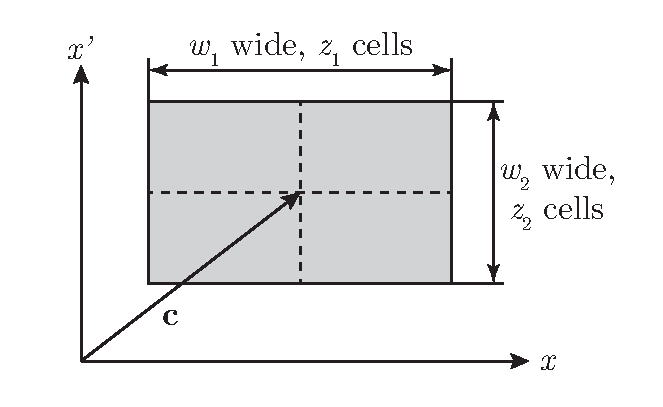
\includegraphics[width=10cm]{fig/state-space-region.pdf}
	\caption{The definition of state space region in $(x,x')$ based on its center $\mathbf{c}$ and width $\mathbf{w}$ with cell count vector $\mathbf{z}$.} \label{fig:statespace}
\end{figure}

\begin{lstlisting}
int main() {
 Pendulum pendulum(1.0, 0.2, 0.1);
 // Cell state space properties
 vec2 center = {0.0, 0.0};
 vec2 width  = {16.0*M_PI, 10.0};
 vector<uint32_t> cells = {1400, 800};
 // SCM object and solution
 SCM32<vec2> scm(center, width, cells, &pendulum);
 scm.solve(20); // Max. number of steps to leave state-space cells
 scm.generateImage("pendulum.jpg");
 return 0;
}
\end{lstlisting}
The \texttt{SCM32<StateVectorType>} class' template parameter in this case is \texttt{vec2} as the \texttt{Pendulum} used that type for the state vector. Note: \texttt{SCM32} is a type definition for \texttt{SCM<SCMCell<uint32\_t>, uint32\_t, StateVectorType>} meaning, that the addressing of cells are done with 32-bit unsigned integers. If your state space contains more than $2^{32}-1 = 4\,\mathrm{GCells}$, use \texttt{SCM64} instead.

After running this example program, the following output is generated:

\begin{figure}[h]
	\centering
	\includegraphics[width=14cm]{fig/pendulum.jpg}
	\caption{\texttt{pendulum.jpg}: the $(\varphi, \dot\varphi)$ state space of the simple pendulum. Coloured regions indicate domains of attraction of stable equilibria -- fixed points.}
\end{figure}

\noindent \emph{Related files}: \texttt{demo-pendulum.cpp, pendulum.h} in the \texttt{demo} folder.

\noindent \emph{Exercise}: Modify the damping parameter of the example and see how the state-space changes.

\newpage

\subsection{Micro-chaos map}

Consider a PD-controlled 1 DoF inverted pendulum, where the quantized control force is calculated at sampling intervals $\tau$ (zero-order hold). According to the solution of the linearised, dimensionless equation of motion, the following so-called \emph{micro-chaos map} can be derived between the states at subsequent sampling instants:
\begin{equation}\label{eq:microchaos}
\mathbf{y}_{i+1}=\mathbf{U}\,\mathbf{y}_i+\mathbf{b} \,F_i,
\end{equation}
where $F_i=\mathrm{Int}(\hat P x_{i}+\hat D x'_{i})$, $\mathbf{y}=[x_i\quad x'_i]^T$, and:

\begin{equation} 
\mathbf{U}=\frac{e^{-\hat{\alpha} \delta}}{\Gamma}
\left[
\begin{array}{cc}
\Gamma  \cosh \left(\hat{\alpha } \Gamma \right)+\delta  \sinh \left(\hat{\alpha } \Gamma  \right) & \sinh \left(\hat{\alpha } \Gamma  \right)/\hat{\alpha } \\
\hat{\alpha } \sinh \left(\hat{\alpha } \Gamma  \right) & \Gamma  \cosh \left(\hat{\alpha } \Gamma  \right)-\delta  \sinh \left(\hat{\alpha } \Gamma  \right) \\
\end{array}
\right], \nonumber
\end{equation}
\begin{equation}
\mathbf{b}=\frac{1}{{\hat\alpha}^2 \Gamma}\left[\begin{array}{cc}
\Gamma -e^{-\hat{\alpha } \delta } \left(\Gamma  \cosh \left(\hat{\alpha } \Gamma  \right)+\delta \sinh \left(\hat{\alpha } \Gamma  \right)\right) \\
-\hat{\alpha} e^{- \hat{\alpha } \delta }\sinh \left(\hat{\alpha } \Gamma  \right)
\end{array}\right] \nonumber
\end{equation}
where $\Gamma=\sqrt{1+\delta^2}$, and $\hat{\alpha}$ is the dimensionless stiffness, $\delta$ is the relative damping and $\hat{P}, \hat{D}$ are the dimensionless control gains. $\mathrm{Int}()$ denotes taking the integer part of the calculated control effort, and thus introduces switching lines for every integer value.

This system is implemented in the \texttt{microchaos.h/cpp} files in the \texttt{demo} folder of the repository. The system class needs to implement the \texttt{step} function of the \texttt{DynamicalSystemBase} class.

\begin{lstlisting}
vec2 MicroChaosMapStatic::step(const vec2& y0) const {
 double F = SymmetricFloor(k*y0); // Rounding at output, k = {P,D}
 vec2 y1 = U*y0 + b*F;            // The micro-chaos map
 return y1;
}
\end{lstlisting}

To apply SCM on this problem, consider the following code snippet:

\begin{lstlisting}
int main() {
 double P = 0.007;        // Parameters and system
 double D = 0.02;
 double alpha = 0.078;
 double delta = 0;
 MicroChaosMapStatic system(P, D, alpha, delta);
 vec2 center = {0, 0};    // State-space properties
 vec2 width  = {2400, 50};
 vector<uint32_t> cells = {1000, 400};
 SCM32<vec2> scm(center, width, cells, &system); // SCM
 scm.solve(20);
 scm.generateImage("scm-microchaos.jpg");
 return 0;
}
\end{lstlisting}
\newpage 
After successful execution, the following output image is generated:

\begin{figure}[h!]
	\centering
	\includegraphics[width=15cm]{fig/microchaos.jpg}
	\caption{SCM results for the micro-chaos map. Coloured regions indicate domains of attraction of chaotic attractors (white cell groups along the $x$ axis).}
\end{figure}

\noindent \emph{Related files}: \texttt{demo-microchaos.cpp, microchaos.h/cpp} in the \texttt{demo} folder.

\noindent \emph{Exercise}: Increase the cell count in the example and see how the tiny details of the state space reveal themselves.

Note: a 4 gigapixel image (corresponding to 4 billion cells, close to the limit of the 32bit unsigned integer address) of this example is hosted at:  \href{http://www.mm.bme.hu/~gyebro/scm/}{mm.bme.hu/$\sim$gyebro/scm/}


\subsection{Duffing oscillator}

Consider the Duffing equation:

\begin{equation}
\ddot x(t) + \delta\,\dot x(t) + \alpha x(t) + \beta x^3(t) = \gamma\,\cos(\omega\,t)
\end{equation}

The implementation of this dynamical system can be found in the \texttt{duffing.h} file. In this example SCM is applied to generate a Poincaré-section of this system by choosing integration time to $T = 2\,\pi / \omega$. \\
Consider the following code snippet:

\begin{lstlisting}
int main() {
 double alpha = -1.0;       // System and its parameters
 double beta  = 1.0;
 double gamma = 0.28;
 double delta = 0.3;
 double omega = 1.2;
 double T = 2*M_PI/omega;
 DuffingOscillator duffing(alpha, beta, gamma, delta, omega, T);
 
 vec2 center = {0.0, 0.0};  // Cell state space properties
 vec2 width  = {4.0, 3.0};
 vector<uint32_t> cells = {1000, 1000};

 SCM32<vec2> scm(center, width, cells, &duffing);
 // Declare an alternate coloring method
 SCMBlackAndWhiteColoring<uint32_t> coloringMethod;
 
 // Execute SCM with different gamma values
 vector<double> gammas = {0.28, 0.29, 0.37, 0.5};
 for (double g : gammas) {
  duffing.setGamma(g);
  scm.solve(20);
  string imageName = "scm-duffing-gamma="+to_string(g)+".jpg";
  scm.generateImage(imageName, &coloringMethod);
 }
 return 0;
\end{lstlisting}

Upon successful execution, multiple output images show some characteristic Poincaré-sections of the Duffing equation.

\begin{figure}[h]
	\centering
	\includegraphics[width=10cm]{fig/duffing.jpg}
	\caption{SCM results for the Duffing oscillator's Poincaré-section at $\gamma = 0.5$.}
\end{figure}

\noindent \emph{Related files}: \texttt{demo-duffing.cpp, duffing.h} in the \texttt{demo} folder.\\
\noindent \emph{Exercise}: Run the demo and examine the other outputs. Play with the state space resolution and other system parameters.

\begin{thebibliography}{99}
	
	\bibitem{HSU87} Hsu, C.S. "Cell-to-Cell Mapping: A Method of Global Analysis for Nonlinear Systems", Springer, Singapore, Applied Math. Sciences, 64, 1987. DOI: \href{https://doi.org/10.1007/978-1-4757-3892-6}{10.1007/978-1-4757-3892-6}
	
	\bibitem{CNSNS16} Gyebr\'oszki, G., Csern\'ak, G. "Clustered Simple Cell Mapping: An extension to the Simple Cell Mapping method", {\em Communications in Nonlinear Science and Numerical Simulation} \textbf{42}: pp. 607-622, 2017. DOI: \href{https://doi.org/10.1016/j.cnsns.2016.06.020}{10.1016/j.cnsns.2016.06.020}
	
\end{thebibliography}

\end{document}